% CVPR 2022 Paper Template
% based on the CVPR template provided by Ming-Ming Cheng (https://github.com/MCG-NKU/CVPR_Template)
% modified and extended by Stefan Roth (stefan.roth@NOSPAMtu-darmstadt.de)

\documentclass[10pt,twocolumn,letterpaper]{article}

%%%%%%%%% PAPER TYPE  - PLEASE UPDATE FOR FINAL VERSION
%\usepackage[review]{cvpr}      % To produce the REVIEW version
\usepackage{cvpr}              % To produce the CAMERA-READY version
%\usepackage[pagenumbers]{cvpr} % To force page numbers, e.g. for an arXiv version

% Include other packages here, before hyperref.
\usepackage{graphicx}
\usepackage{amsmath}
\usepackage{amssymb}
\usepackage{booktabs}


% It is strongly recommended to use hyperref, especially for the review version.
% hyperref with option pagebackref eases the reviewers' job.
% Please disable hyperref *only* if you encounter grave issues, e.g. with the
% file validation for the camera-ready version.
%
% If you comment hyperref and then uncomment it, you should delete
% ReviewTempalte.aux before re-running LaTeX.
% (Or just hit 'q' on the first LaTeX run, let it finish, and you
%  should be clear).
\usepackage[pagebackref,breaklinks,colorlinks]{hyperref}


% Support for easy cross-referencing
\usepackage[capitalize]{cleveref}
\crefname{section}{Sec.}{Secs.}
\Crefname{section}{Section}{Sections}
\Crefname{table}{Table}{Tables}
\crefname{table}{Tab.}{Tabs.}


%%%%%%%%% PAPER ID  - PLEASE UPDATE
\def\cvprPaperID{*****} % *** Enter the CVPR Paper ID here
\def\confName{CVPR}
\def\confYear{2022}

\graphicspath{{./figures/}}
\begin{document}

%%%%%%%%% TITLE
\title{Generating Expressive Facial Mesh Animation : A Survey}

\author{
HJW\\
Institution1 address\\
{\tt\small ykn@rtfm.moe}
% For a paper whose authors are all at the same institution,
% omit the following lines up until the closing ``}''.
% Additional authors and addresses can be added with ``\and'',
% just like the second author.
% To save space, use either the email address or home page, not both
}
\maketitle

%%%%%%%%% ABSTRACT
\begin{abstract}
With technology allowing for increasing realism in games and movies, facial animation is still a very challenging task. 

"Lorem ipsum dolor sit amet, consectetur adipiscing elit, sed do eiusmod tempor incididunt ut labore et dolore magna aliqua. Ut enim ad minim veniam, quis nostrud exercitation ullamco laboris nisi ut aliquip ex ea commodo consequat. Duis aute irure dolor in reprehenderit in voluptate velit esse cillum dolore eu fugiat nulla pariatur. Excepteur sint occaecat cupidatat non proident, sunt in culpa qui officia deserunt mollit anim id est laborum."
\end{abstract}

%%%%%%%%% BODY TEXT
\section{Introduction}
\label{sec:intro}

Facial animation can be applied to various fields.

Psychologically, Human tend to be very sensitive to facial motion. Slightest uncanniest in facial animation is directly lead to hurt overall experience of embodiment, and overall experience\cite{hansonUpendingUncannyValley}. So, delivering natural expressive facial animation is a great interest in graphics field.

To achieve realistic 3D face animation naturally, high-quality animation is required. Animating high-quality expressive face is very labor-intensive job when done by animator. Another approach is to capture human face animation in 3D. Face capture is a well-understood field(cite here), yet such approach requires gigabytes of data from expensive capture system, and is hard to manipulate. Therefore, it is necessary to simplify such process. 

To simplify such process, one can automatically generate facial animation or can simplify animating produce.

In this survey, I introduce and compare three research that animate expressive facial animation :
\begin{itemize}
 \item JALI\cite{edwardsJALIAnimatorcentricViseme2016} and VisimeNet\cite{zhouVisemenetAudiodrivenAnimatorcentric2018}, a linguistic approach to lip-sync.
 \item MeshTalk\cite{richardMeshTalk3DFace2021}, a deep learning method.
 \item D3DExpression\cite{potamiasLearningGenerateCustomized2020}, LSTM method which replicate facial expression.
\end{itemize}


% Creating lip-sync animation is complex and challenging task.

% Mapping face expression to latent space is actively being researched due to recent advancement in deep learning field.



\section{Methods}

\subsection{JALI and VisimeNet}

\begin{figure}
   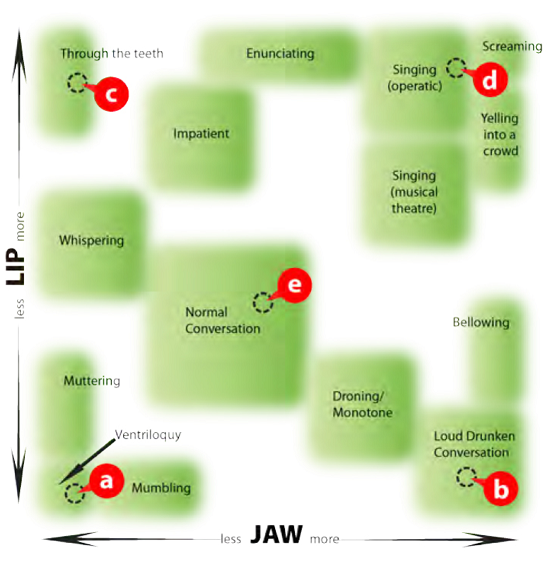
\includegraphics[width=1.0\linewidth]{jaliStyles}
   
   \caption{Speaking styles of JALI viseme field}
   \label{fig:jaliStyles}
\end{figure}

Creating lip-sync animation is complex and challenging task. Lip-sync is traditionally done by linguistic approach. Mapping text to phonemes, then visemes, the position of lip and jaw\cite{ezzatMikeTalkTalkingFacial1998}. Phonemes to visemes is a complex many-to-many mapping.

JALI\cite{edwardsJALIAnimatorcentricViseme2016} is a state of the art viseme model. JALI takes jaw and lip activation multipliers into consideration, since jaw and lip is the most significant acoustic motion in face.

JALI many-to-one map phonemes to viseme. Then applied animated jaw-lip multipliers to the face.

As shown on \cref{fig:jaliStyles}, different speaking styles shows different jaw lip activation level multipliers. Which can be animated more intuitively.

JALI model requires manual labor such as aligning audio to plain text or phonemes. This lead to research to automate such process. This approach requires extracting viseme and jaw-lip model sequence from audio. 



%Creating lip-sync animation from audio signal only is an attractive approach since it does not require any costly camera or tracking device. 

%Eye and eyebrow animation is another topic.

%Capturing and mapping to latent space is a field.

%Emotion transition from/to neutral face is a field.


%%%%%%%%% REFERENCES
{\small
\bibliographystyle{ieee_fullname}

\bibliography{refs}
}

\end{document}
